\subsubsection{Delete and shift}
After $B$ extracts the public key of $C$, it deletes the routing information from the packet. $B$ then fills the empty space with its own blinding (which is different from the one received from $A$) by setting the key share $\alpha_0$ to $\alpha_1=g^{xb_0}$. $B$ also computes $\beta_1$ as follows:

\begin{comment}
\begin{figure}[H]
    \centering
    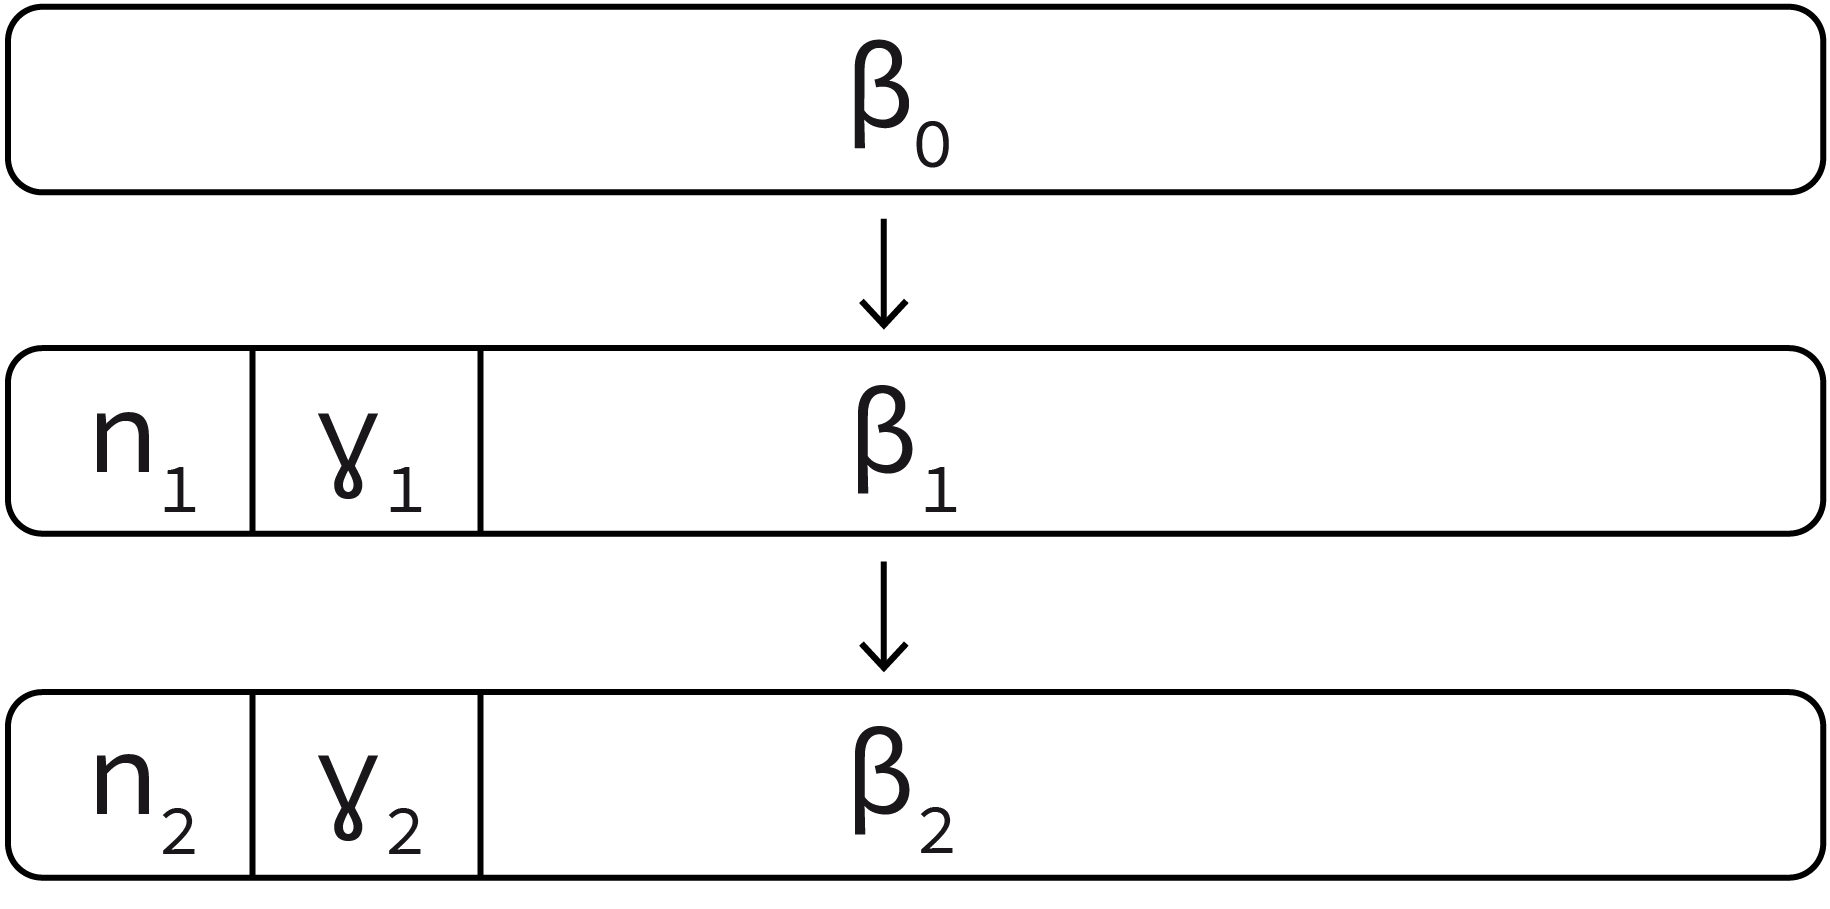
\includegraphics[width=6cm,height=6cm,keepaspectratio]{../yellowpaper/images/FigureB.png}
    \caption{The processing of the routing information $\beta$}
    \label{fig:The processing of the routing information beta}
\end{figure}
\end{comment}

The first $\kappa$ bits of $\beta_0$ will be $n_{1}$ itself, the next $\kappa$ bits will be $\gamma_{1}$, and the remaining $(2r-1)\kappa$ bits of $\beta_0$ are shifted left to form the leftmost $(2r-1)\kappa$ bits of $\beta_{1}$; the rightmost $2\kappa$ bits of $\beta_{1}$ are simply a substring of an output of the PRG function.

The new mix header is now ready to be sent to $C$, defined as the node with public key $y_1$:

$$M_1=(\alpha_1,\beta_1,\gamma_1)$$

where $\alpha$, $\beta$ and $\gamma$ are defined in equations $\ref{eq:1}$, $\ref{eq:2}$ and $\ref{eq:6}$